\section{Auswertung}
\label{sec:Auswertung}
Die Fehler werden mittels Python und der Gaußschen Fehlerfortpflanzung berechnet,
\begin{equation}
\Delta f=\sqrt{\sum_{i=1}^N\left(\frac{\text{d}f}{\text{d}y_i}\right)^2(\Delta y_i)^2}.
\label{eq:Gauß}
\end{equation}
$f$ ist dabei unsere zur Berechnung nötige Funktion, $y$ unsere Variablen und $\Delta y$ deren Abweichung.
\subsection{Druck unter einem Bar}
\begin{table}
  \centering
  \caption{Temperatur und Druck bei Verdampfung des Wassers. Der Druck hat eine Messunsicherheit von
  $\pm1$mB, die Temperatur von $\pm 1$ K.}
  \label{tab:Messreihe_1}
  \begin{tabular}{
  c c c||c c c||c c c
}
\toprule 
$T\,/ \unit{\kelvin}$ & $T\,/ \unit{\celsius}$ & $p\,/ \text{mbar}$ &
$T\,/ \unit{\kelvin}$ & $T\,/ \unit{\celsius}$ & $p\,/ \text{mbar}$ &
$T\,/ \unit{\kelvin}$ & $T\,/ \unit{\celsius}$ & $p\,/ \text{mbar}$ \\
\midrule
293.15 & 20 & 40  & 320.15 & 47 & 421 & 347.15 & 74 & 690 \\
294.15 & 21 & 167 & 321.15 & 48 & 431 & 348.15 & 75 & 701 \\    
295.15 & 22 & 228 & 322.15 & 49 & 439 & 349.15 & 76 & 716 \\                      
296.15 & 23 & 255 & 323.15 & 50 & 445 & 350.15 & 77 & 723 \\      
297.15 & 24 & 274 & 324.15 & 51 & 453 & 351.15 & 78 & 743 \\      
298.15 & 25 & 287 & 325.15 & 52 & 461 & 352.15 & 79 & 760 \\      
299.15 & 26 & 296 & 326.15 & 53 & 465 & 353.15 & 80 & 773 \\      
300.15 & 27 & 303 & 327.15 & 54 & 476 & 354.15 & 81 & 790 \\     
301.15 & 28 & 310 & 328.15 & 55 & 482 & 355.15 & 82 & 810 \\  
302.15 & 29 & 316 & 329.15 & 56 & 491 & 356.15 & 83 & 826 \\  
303.15 & 30 & 322 & 330.15 & 57 & 500 & 357.15 & 84 & 844 \\
304.15 & 31 & 327 & 331.15 & 58 & 511 & 358.15 & 85 & 856 \\
305.15 & 32 & 331 & 332.15 & 59 & 520 & 359.15 & 86 & 879 \\
306.15 & 33 & 336 & 333.15 & 60 & 528 & 360.15 & 87 & 901 \\
307.15 & 34 & 341 & 334.15 & 61 & 537 & 361.15 & 88 & 913 \\
308.15 & 35 & 347 & 335.15 & 62 & 549 & 362.15 & 89 & 933 \\ 
309.15 & 36 & 351 & 336.15 & 63 & 562 & 363.15 & 90 & 944 \\
310.15 & 37 & 356 & 337.15 & 64 & 571 & 364.15 & 91 & 966 \\
311.15 & 38 & 362 & 338.15 & 65 & 578 & 365.15 & 92 & 979 \\
312.15 & 39 & 367 & 339.15 & 66 & 586 & 366.15 & 93 & 990 \\
313.15 & 40 & 372 & 340.15 & 67 & 600 & 367.15 & 94 & 1015\\
314.15 & 41 & 379 & \text{--} &  &    & 368.15 & 95 & 1030\\
315.15 & 42 & 385 & 342.15 & 69 & 628 & 369.15 & 96 & 1046\\
316.15 & 43 & 395 & 343.15 & 70 & 638 & 370.15 & 97 & 1061\\
317.15 & 44 & 400 & 344.15 & 71 & 650 & 371.15 & 98 & 1079\\
318.15 & 45 & 405 & 345.15 & 72 & 660 & 372.15 & 99 & 1093\\
319.15 & 46 & 412 & 346.15 & 73 & 670 & 373.15 & 100 & 1108 \\
\bottomrule
\end{tabular}
\end{table}
\begin{table}[H]
  \centering
  \caption{Temperatur und Druck bei Verdampfung des Wassers für $p\geq 1$.Der Druck hat eine Messunsicherheit von
  $\pm1$\,mbar, die Temperatur von $\pm 1$\,K.}
  \label{tab:Messreihe_2}
\begin{tabular}{
  c c||c c
}
\toprule 
$p$/\,bar & $T$/\,K & $p$/\,bar & $T$/\,K\\
\midrule
1000  & 391.15 & 9000  & 447.15\\
2000  & 404.15 & 10000 & 451.15\\
3000  & 413.15 & 11000 & 454.15\\
4000  & 419.15 & 12000 & 459.15\\
5000  & 427.15 & 13000 & 461.15\\
6000  & 433.15 & 14000 & 463.15\\
7000  & 438.15 & 15000 & 465.15\\
8000  & 443.15 &       &      \\
\bottomrule
\end{tabular}
\end{table}
Mit diesen gemessenen Werten lassen sich folgende Grafiken erstellen. $p_0$ ist hierbei gleich 1\,bar.
\begin{figure}[H]
  \begin{subfigure}{0.48\textwidth}
      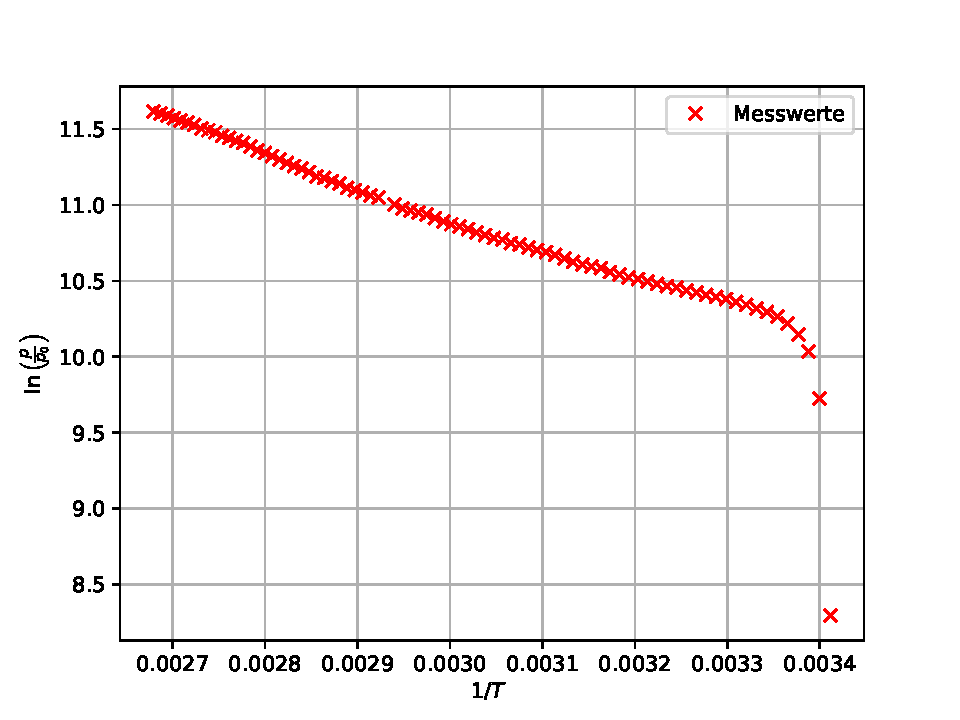
\includegraphics[height=6cm]{plota.pdf}  
    \caption{Bereich von $30$ bis $\SI{1000}{\milli\bar}$.}
    \label{fig:MesswerteKlein}
  \end{subfigure}
  \hfill
  \begin{subfigure}{0.48\textwidth}
    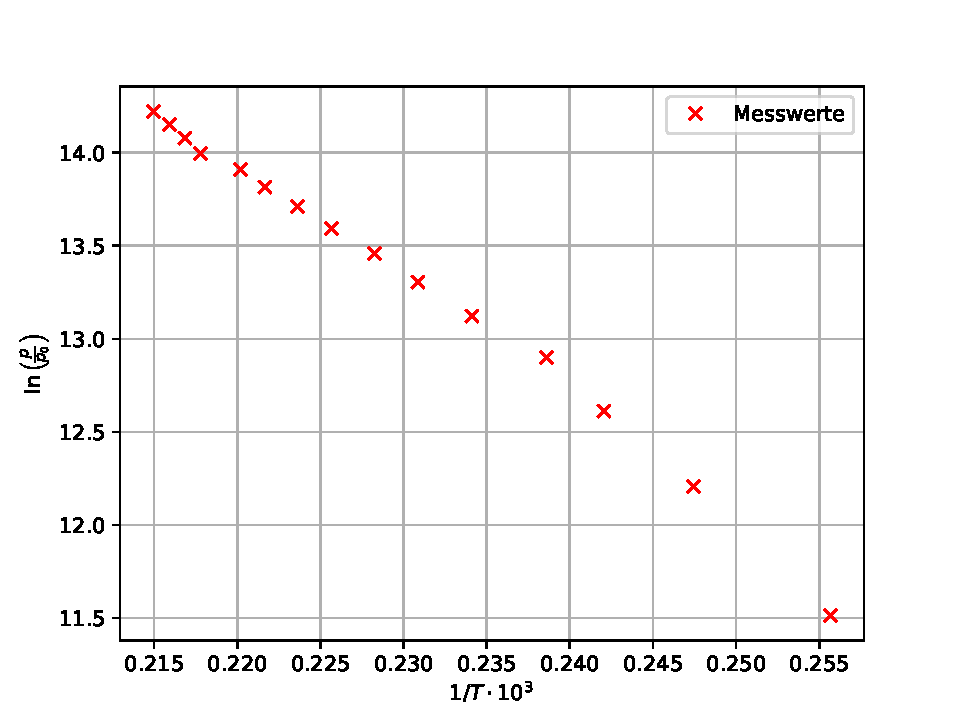
\includegraphics[height=6cm]{plotb.pdf}
    \caption{Bereich von $1$ bis $\SI{15}{\bar}$.}
    \label{fig:MesswerteGross}
  \end{subfigure}
  \caption{Die Messwerte beider Messreihen aufgetragen als der Logarithmus des Drucks $p$
  gegen die reziproke absolute Temperatur $T$.}
  \label{fig:Teila}
\end{figure}
\noindent
Die Messwerte wurden in Grad Celsius aufgenommen, für die Auswertung jedoch in Kelvin umgerechnet. Außerdem wurden die ersten beiden Messwerte ausgelassen,
da sie offensichtlich deutlich von den restlichen Werte abwichen.
Um daraus die zu berechnende Verdampfungswärme des Wassers zu bestimmen, wird eine Gerade durch die Messwerte gelegt.
Diese wird mittels Python für den Bereich von $30$ bis $1000$\,mbar erstellt. \\
\begin{figure}[H]
  \centering
  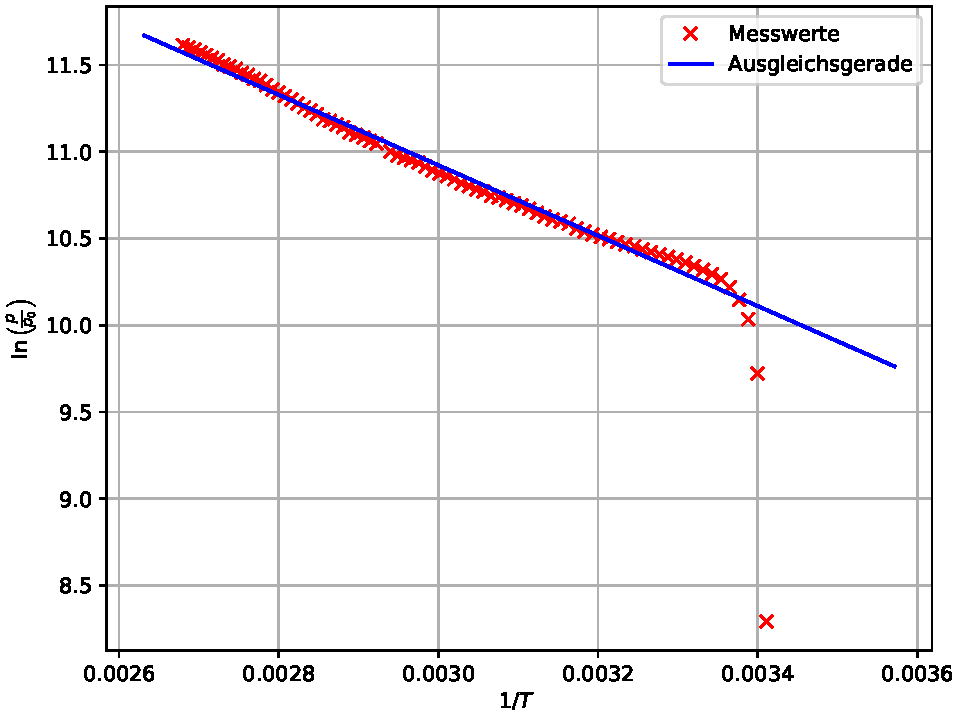
\includegraphics[scale=0.8]{plotc.pdf}
  \caption{Die Messwerte der ersten Messreihe aufgetragen als der Logarithmus des Drucks $p$
  gegen die reziproke absolute Temperatur $T$ mit der Ausgleichsgerade. $p_0=1$\,bar.}
  \label{fig:Ausgleichsgerade}
\end{figure}\noindent
Die Gleichung zur Bestimmung von $L$ und dem damit einhergehenden Fit ist wie folgt:
\begin{equation}
  \ln(p) = - \frac{L}{R} \cdot \frac{1}{T}
  \Rightarrow y = a \cdot x + b = -2029 \cdot x + 5,497
\end{equation}
Mit numeric Python und Gl.\eqref{eq:Gauß} ergeben sich folgende Messunsicherheiten: $a = \SI{2029 +- 21}{\kelvin}$
und $b = \SI{5.497 \pm 0.063}{\elvin}$.
Die Verdampfungswärme wird mit folgendem Wert berechnet:
\begin{equation*}
  L = - \ a \cdot R \Rightarrow L = \SI{1.69(0.02)e4}{\joule\per\mol}
\end{equation*}
$R$ ist die allgemeine Gaskonstante mit einem Wert von $\SI{8.314}{\joule\per\mole\per\kelvin}$\,\cite{Gaskonstante}.
$L$ ist die Steigung der Ausgleichsgeraden in Abbildung \ref{fig:Ausgleichsgerade} multipliziert mit der Universellen Gaskonstante $R$.
\noindent
Jetzt soll die äußere Verdampfungswärme $L_a$ bestimmt werden.
Diese beschreibt die benötigte Arbeit, um bei konstantem Druck das Volumen eines Stoffs zu verändern.
Hierfür wird die ideale Gasgleichung verwendet, die für ideale Gase genau diese Arbeit angibt,
\begin{equation}
    p \cdot V = R \cdot T = L_a
\end{equation}
Also ergibt sich $L_a = \SI{3101.3}{\frac{\J}{\mol}}$.
Um die erforderliche Arbeit zur Überwindung der molekularen Anziehungskraft bei Verdampfung $L_i$ zu bestimmen, wird
zunächst die Differenz zwischen $L$ und $L_a$ gebildet.
\begin{equation}
    L_i = L - L_a \Rightarrow L_i = \SI{13800 \pm 170}{\frac{\J}{\mol}}
\end{equation}
Um hier raus jetzt die Kraft für ein Molekül auszurechnen, muss die Definition für ein Mol eingesetzt werden.
Also muss $L_i$ durch die Avogadro-Konstante $N_a = \SI{6.022e23}{\per\mol}$ \cite{Avogadro} geteilt werden.
Zuletzt muss noch die Einheit in eV umgerechnet werden.
\begin{equation*}
  L_i = \SI{0.1430 \pm 0.0018 }{eV}
\end{equation*}

\subsection{Druck über einem Bar}
Auflösen der Clausius-Clapeyronschen Gleichung nach $L$ zur Bestimmung der Wärmeabhängigkeit ergibt.\\
\begin{align}
  &(V_D-V_F)\text{d}p=\frac{L}{T}\text{d}T\nonumber\\
  \Leftrightarrow L=&(V_\text{D}-V_\text{F})\frac{\text{d}p}{\text{d}T}T\label{eqn:L(V,T)}
\end{align}
Mittels Python und scipy wird polynomialer Fit dritten Grades errechnet. Die 
zum Polynom $p(T)=a\cdot T^3+b\cdot T^2+c\cdot T+d$ gehörenen Vorfaktoren sind:
\begin{align*}
  a &= \num{2.1(0.6)e-5}\,\si{\bar\per\kelvin\cubed}\\
  b &= (-0.02 ± 0.008)\,\si{\bar\per\kelvin\squared}\\
  c &= (9.9 ± 3.3)\,\si{\bar\per\kelvin}\\
  d &= \num{-1.33(0.47)e3}\,\si{\bar}\\
\end{align*}
Abbildung \ref{fig:Druck_groß} zeigt den Plot mit den errechneten Werten.
\begin{figure}[H]
\centering
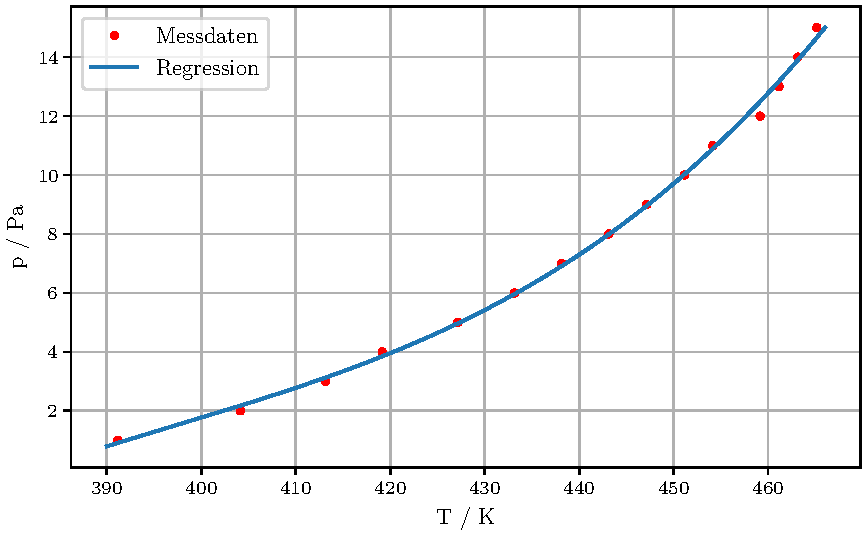
\includegraphics[height=7cm]{plotd.pdf}
\caption{Druck und Temperatur der zweiten Messreihe, $p\geq 1$\,bar, sowie 
der Fit durch die Messwerte.}
\label{fig:Druck_groß}
\end{figure}
Ableitung des Polynoms $p(T)$ ergibt
\begin{equation}
p'(T)=3\cdot a\cdot T^2+2\cdot b\cdot T+c.
\end{equation}
Das ist der Ausdruck für $\frac{\text{d}p}{\text{d}T}$.In der Theorie wurde unter einer Bedingung die Annahme getroffen, dass $V_F$ gegen $V_D$
vernachlässigt werden darf. Dies wird hier genutzt. Nach Umstellen der Formel aus der Theorie ergibt sich für $V=V_\text{D}$:
\begin{align}
   RT&=\left(p+\frac{a}{V^2}\right)V\\
   \intertext{a ist hierbei gleich 0,9\,$\text{J m}^3\text{mol}^{-2}$.}
   \intertext{Mithilfe der pq-Formel ergibt sich}
   \Rightarrow V&=\frac{RT}{2p}\pm\sqrt{\left(\frac{RT}{2p}\right)^2+\frac{a}{p}}\label{eqn:V(T)}
   \intertext{Durch einsetzen von Gl.\eqref{eqn:V(T)} in Gl.\eqref{eqn:L(V,T)} lässt sich folgender Ausdruck für L finden:}
   L(T)&=\frac{T}{P}\left(\frac{RT}{2}\pm\sqrt{\left(\frac{R^2T^2}{4}\right)-ap}\right).
\end{align}
In Abbildung \ref{fig:Verdampfungswärme} wird $L(T)$ mit Python geplottet.
\begin{figure}
  \label{fig:Verdampfungswärme}
  \begin{subfigure}{0.45\textwidth}
  \centering
  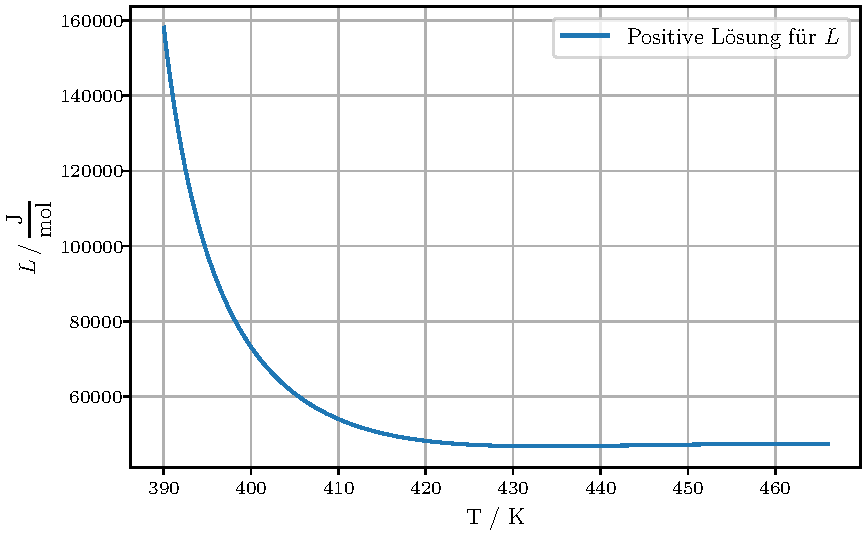
\includegraphics[height=4cm]{plote.pdf}
  \caption{$L$ in Abhängigkeit von T für $V_{D+}$.}
  \label{fig:Verdampfungswärme1}
  \end{subfigure}
  \hfill
  \begin{subfigure}{0.45\textwidth}
  \centering
  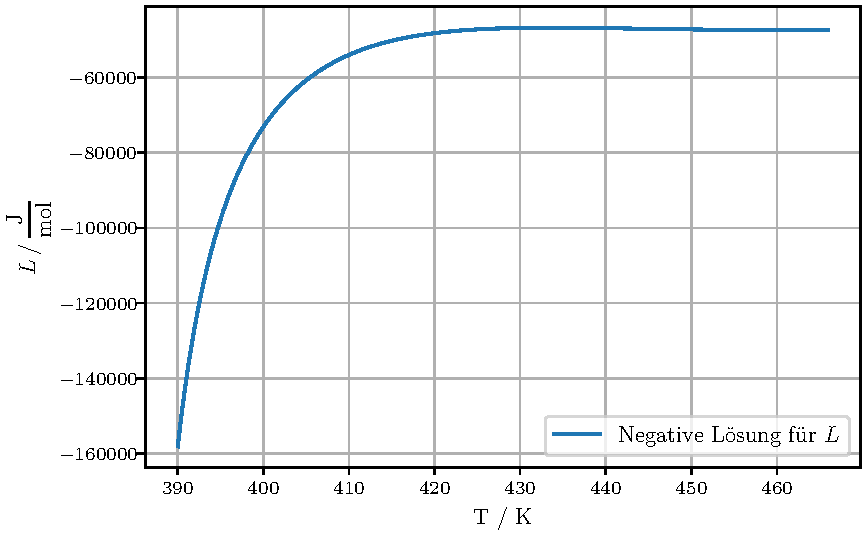
\includegraphics[height=4cm]{plotf.pdf}
  \caption{$L$ in Abhängigkeit von T für $V_{D-}$.}
  \label{fig:Verdampfungswärme2}
  \end{subfigure}
  \caption{Das Ergebnis für positivie Werte ist das physikalisch sinnvolle, da eine negative 
  Energie bzw. Verdampfungswärme nicht aufgebracht werden kann.}
\end{figure}
